\documentclass{mwart}

\usepackage[utf8]{inputenc}
\usepackage{polski}
\usepackage{booktabs}
\usepackage{url}
\usepackage{graphicx}
\usepackage{bbding}

\newcommand*\tick{\item[\Checkmark]}
\newcommand*\fail{\item[\XSolidBrush]}

\author{Tomasz Dwojak, Marcin Żurowski}
\title{Wprowadzenie do języków skryptowych: Python}
\date{\today}

\begin{document}
\maketitle

\section{Cel zajęć}
Celem lekcji jest przedstawienie i nauczenie podstawowych elementów języka Python.
Obecnie jest to najpopularniejszy język skryptów, który posiada wiele pakietów, np. do
analizy danych. Program lekcji zakłada, że uczestnicy posiadają minimalne
doświadczenie programistyczne. Z tego powodu pominięty został materiał wprowadzający do
programowania imperatywnego.

\section{Wymagania}
\begin{itemize}
  \item Minimalne doświadczenie z innymi językami programowania,
  \item komputer z dowolnym systemem operacyjnym: Linux, Windows, OS X.
  \item Dostęp do internetu.
\end{itemize}


\section{Rozkład zajęć}

\begin{center}
  \begin{tabular}{p{10cm}r}
  \toprule
  \textbf{Element zajęć}  & \textbf{Czas (w min.)}   \\
  \midrule
  Języki kompilowane  a skryptowymi: różnice, wady i zalety języków skryptowych. & 5 \\
  \midrule
  Wprowadzenie do środowiska pracy - IPython notebook: uruchomienie środowiska, omówienie
  komórki i podstawowych funkcjonalności, uruchomienie kodu znajdującego się w komórce.
  & 5 \\
  \midrule
  Uruchomienie przykładowej notebooka & 5 \\
  \midrule
  Wprowadzenie podstawowych elementów języka: operacje arytmetyczne, wyświetlanie,
  posługiwanie się zmiennymi. & 10 \\
  \midrule
  Zadanie z podstawowych elementów (4-5 zadań) & 20 \\
  \midrule
  Wprowadzenie łańcuchów znakowe: tworzenie, modyfikacja, konkatenacja, wyszukiwanie w
  łańcuchu znakowych. & 5 \\
  \midrule
  Zadanie z łańcuchów znaków (5 zadań) & 20 \\
  \midrule
  Listy jako odpowiednik tablic: indeksowanie, tworzenie podlist, dodanie i usuwanie
  elementów, wyszukiwanie elementów. & 10 \\
  \midrule
  Zadanie z list (3 zadań) & 15 \\
  \midrule
  Zadania domowe (3 zadań) & \\
  \bottomrule
\end{tabular}
\end{center}

\section{Materiały}
Cześć materiałów do zajęć znajduje się w repozytorium, które jest dostępne pod adresem
\url{github.com/tomekd/intro_to_python}.

\subsection{Języki skryptowe}
\begin{center}
  \begin{tabular}{lr}
    \toprule
    Forma & Filmik lub artykuł \\
    \midrule
    Czas & 5 minut \\
    Cel & Uświadomienie różnic pomiędzy języka skryptowymi a kompilowalnymi. \\
    \bottomrule
  \end{tabular}
\end{center}

\subsubsection{Wstęp}
Języki programowania możemy podzielić ze względu na sposób uruchomienia na dwie grupy:

\begin{itemize}
  \item języki skryptowe,
  \item języki kompilowane.
\end{itemize}

\subsubsection{Język skryptowy}
W języku skryptowym program jest przechowywany w postaci kodu źródłowego. Podczas
uruchomienia programu kod jest czytany przez program zwany interpreterem. Interpreter
tłumaczy linijka po linijce kod programu na kod maszynowy, a następnie wykonuje go.

\begin{center}
  \begin{figure}
    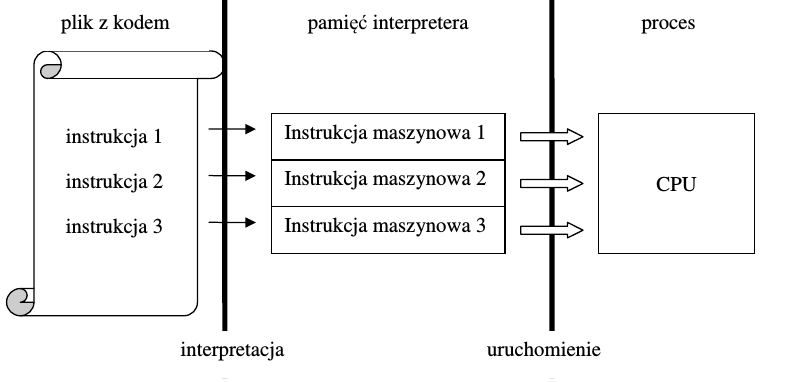
\includegraphics[width=10cm]{diag1}
    \caption{Wypełniony arkusz wprowadzający.}
  \end{figure}
\end{center}

\begin{center}
  \begin{figure}
    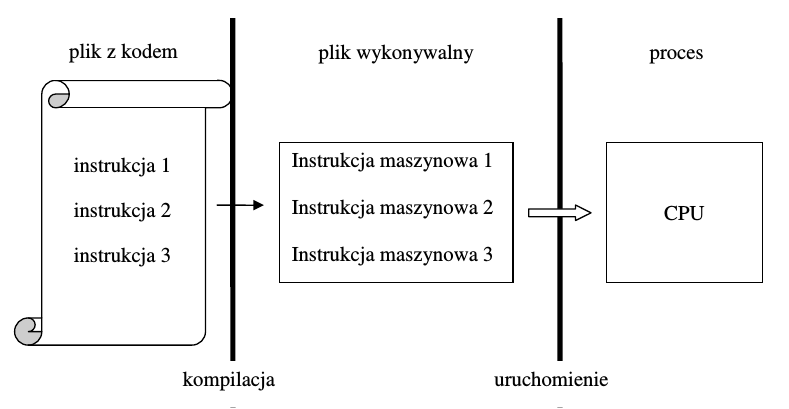
\includegraphics[width=10cm]{diag2}
    \caption{Wypełniony arkusz wprowadzający.}
  \end{figure}
\end{center}

\begin{itemize}
    \tick Szybciej piszę się proste aplikacje,
    \tick Często mniej ścisła składnia, pozwala na pewne ustępstwa,
    \tick Pozwala szybciej poprawiać błędy, używać metody prób i błędów,
    co pomaga przy nauce języka,
    \fail Duże projekty są trudne do utrzymania,
    \fail Mało wydajne,
    \fail Często pozwala na mieszanie kodu z elementami interfejsu, co prowadzi 
    do nieczytelnego kodu,
    \fail Wykrywanie błędów w czasie wykonania wymaga zauważenia niewłaściwego zachowania się
    programu i jest trudne do wykrycia.
\end{itemize}

\subsubsection{Język kompilowalny}
W języku kompilowanym kod programu jest tłumaczony na język maszynowy z pomocą programu
Język kompilowany
zwanego kompilatorem. Program jest przechowywany w postaci kodu maszynowego.
\begin{itemize}
    \tick Wydajne, szybkie i łatwo skalowalne,
    \tick W wielu przypadkach bardziej wydajne od języków skryptowych,
    \tick Często separuje kod od interfejsu, wspierając przejrzystość kodu,
    \tick Za wykrywanie większości błędów odpowiedzialny jest kompilator, który wykrywa
    większość błędów,
    \fail Napisanie aplikacji wymaga więcej pracy niż z językami skryptowymi,
    \fail Bardzo ścisła składnia, wymaga dokładnego programowania,
    \fail Przed uruchomieniem wymagana jest kompilacja, co w dużych projektach wydłuża czas
    znalezienia błędu.
\end{itemize}

\subsubsection{Podsumowanie}
Należy tutaj wspomnieć, że opisane dwie grupy języków nie wskazują, że języki z jednej
grupy są lepsze od języków z drugiej grupy, i języki z jednej grupy należy używać, a
języków z drugiej grupy należy unikać.

\begin{center}
  \begin{tabular}{ll}
    \toprule
    Skryptowe & Ko \\
    \midrule
    Czas & 3 minuty \\
    Cel & Instalacja środowiska pracy potrzebnego podczas całego kursu. \\
    \bottomrule
  \end{tabular}
\end{center}


\subsection{Instalacja środowiska pracy}

Materiał zawarty w tej sekcji jest opcjonalny i jest skierowany głównie do użytkowników systemu
Windows.
\begin{center}
  \begin{tabular}{lr}
    \toprule
    Forma & Screen cast \\
    \midrule
    Czas & 3 minuty \\
    Cel & Instalacja środowiska pracy potrzebnego podczas całego kursu. \\
    \bottomrule
  \end{tabular}
\end{center}

\subsubsection{Scenariusz}

\begin{itemize}
  \item Instalacja środowiska pracy jest bardzo prosta. Istnieją już gotowe programy,
    które zawierają interpreter języka Python oraz zestaw bibliotek, z których będziemy
    korzystać.
  \item Jednym z takich programów jest Anaconda. Wchodzimy na stronę
    \url{www.continuum.io} i przechodzimy do podstrony ''Downloads''. Na stronie możemy
    znaleźć instrukcję instalacji do wszystkich systemów operacyjnych. My skupimy się
    na systemie Windows, ponieważ jest najmniej dostosowany do języków skryptowych.
  \item Przechodzimy do sekcji ''Anaconda for Windows'' i wybieramy wersję "Python-3.5".
  \item Program zaczyna się ściągać, trwa to od 1 do 5 minut.
  \item Program ''Anaconda'' już jest na dysku, możemy przejść do jego instalacji.
  \item Pokazujemy, że należy klikać ''next''. Sama instalacja trwa również do 5 minut.
  \item Świetnie. Anaconda została zainstalowana. Możemy sprawdzić, czy wszystko działa,
    wybierając z ''Start'' $\rightarrow$ ''Anaconda'' $\rightarrow$ ''Jupyter Notebook''.
  \item Uruchamiamy program. Po chwili otwiera się przeglądarka internetowa.
  \item Wszystko działa jak powinno. Możemy zacząć pracę z Pythonem.
\end{itemize}

\begin{center}
  \begin{figure}
  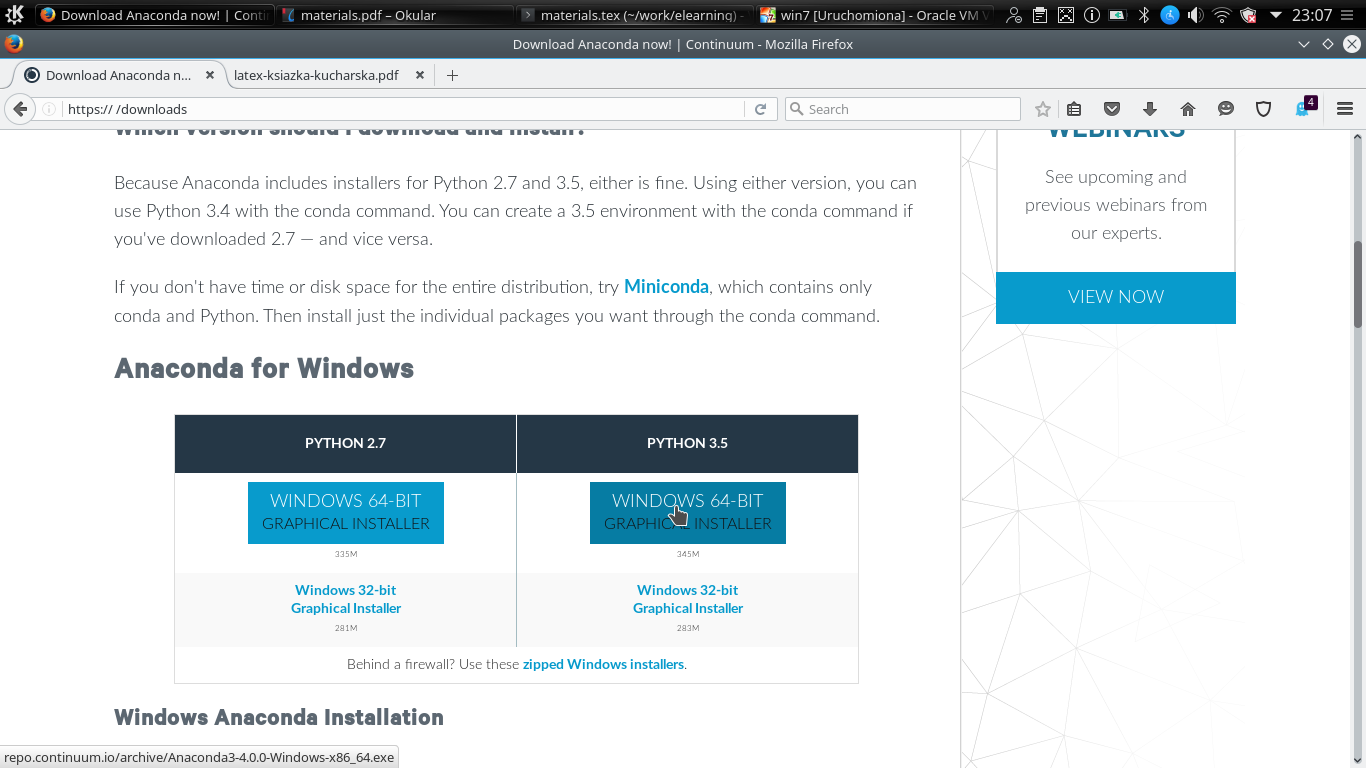
\includegraphics[width=10cm]{install_begin}
  \caption{Strona Anacondy. Kursor wskazuje odpowiedni plik do ściągnięcia.}
  \end{figure}
  \begin{figure}
    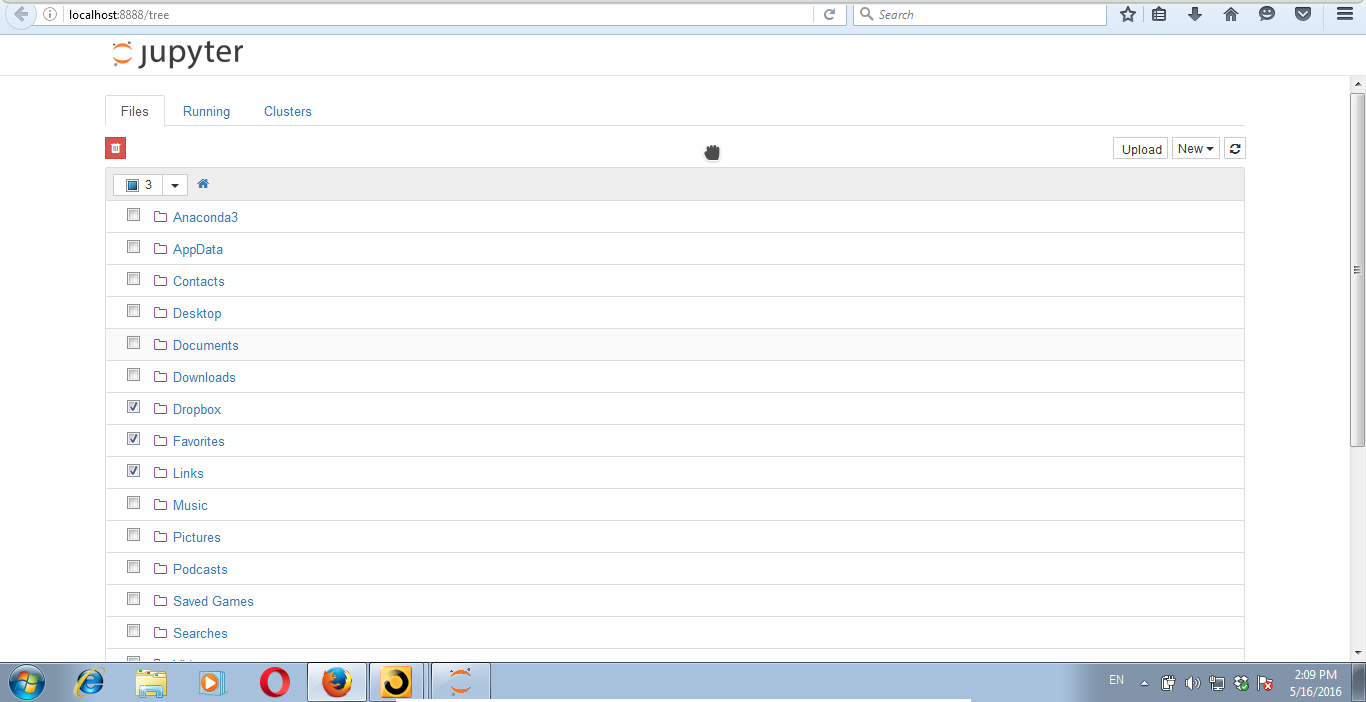
\includegraphics[width=12cm]{install_final}
    \caption{Działający w firefoksie Jupyter Notebook.}
  \end{figure}
\end{center}

\subsection{Pierwsze uruchomienie środowiska}
\begin{center}
  \begin{tabular}{lr}
    \toprule
    Forma & Screen cast \\
    \midrule
    Czas & 3 minuty \\
    Cel & Zapoznanie uczestnika z środowiskiem pracy. \\
    \bottomrule
  \end{tabular}
\end{center}

\subsubsection{Scenariusz}
Końcowy notebook znajduje się w repozytorium: \texttt{notebooks/introToNotebook.ipynb}
\begin{itemize}
  \item Uruchamiamy \texttt{Ipython Notebook}. Po chwili otwiera sie przeglądarka wraz z
    stroną.
  \item Tworzymy nowy notebook i ustawiamy jego nazwę na "Wprowadzenie do Ipython
    Notebook".
  \item Podstawowym elementem notebooka jest komórka (ang. \emph{cell}), do której
    wpisujemy kod naszego programu. Wpiszmy pierwszy kod do komórki:
    \texttt{print("Hello World!")} i wciśnijmy kombinację "Shift + Enter".
  \item Wykonał się kod znajdujący się w komórce.
  \item Widzimy efekt kodu, który był w komórce. Od razu została stworzona nowa pusta
    komórka. Tutaj ponownie możemy wpisać tekst, który zostanie wyświetlony.
  \item Mamy 2 typy komórek, który wybieramy poprzez wybranie z listy znajdującej się w
    \texttt{Cell/Cell Type}. Dwa typy kómórek to \emph{Code} oraz \emph{Markdown}. W
    zależności od typu komórki, kod znajdujący się w komórce zostanie inaczej
    zintepretowany.
  \item Zmieńmy typ komórki na \texttt{Markdown}. Bardzo często chcemy dopisać
    komentarz, który zawiera tekst matematyczny. Z Ipythonem, to nic trudnego: dzięki
    \emph{MathJaksowi} mamy dostęp do Latexa!
  \item Należy powiedzieć, żę Notebook stanowi jedną całość: zmienne i funkcje
    zdefiniowane w jednej komórce są dostępne w następych.
\end{itemize}

\subsubsection{Zadania}
\begin{enumerate}
  \item Ściągnij z repozytorium notebook \texttt{svd.ipynb}. Notebook zawiera zadania z
    rozkładu macierzy SVD. Jeżeli nie wiem, co to jest, to nie musisz się ty przejmować
    -- nie jest to istotne.
  \item Uruchom kod znajdujący się w komórkach.
  \item Spróbuj wykonać kod w komórkach dwoma skrótami: \texttt{Ctrl + Enter} i
    \texttt{Shift + Enter}. Czy widzisz różnicę w zachowaniu?
  \item Zamień kolejnością dwie ostatnie komórki.
  \item Dodaj jako drugą komórkę, nową komórkę typu \emph{Markdown} i wstaw tekst:
    Niech dana będzie macierz A.
  \item Dodaj do nowostworzonej komórki kod Latexa, który wyświetli macierz A.
  \item Z menu \texttt{Cell} wybierz opcję wyczyszczenia wszystkich wyjść. Czy możemy
    teraz w dowolnej kolejności wywoływać komórki?
\end{enumerate}

\begin{center}
  \begin{figure}
    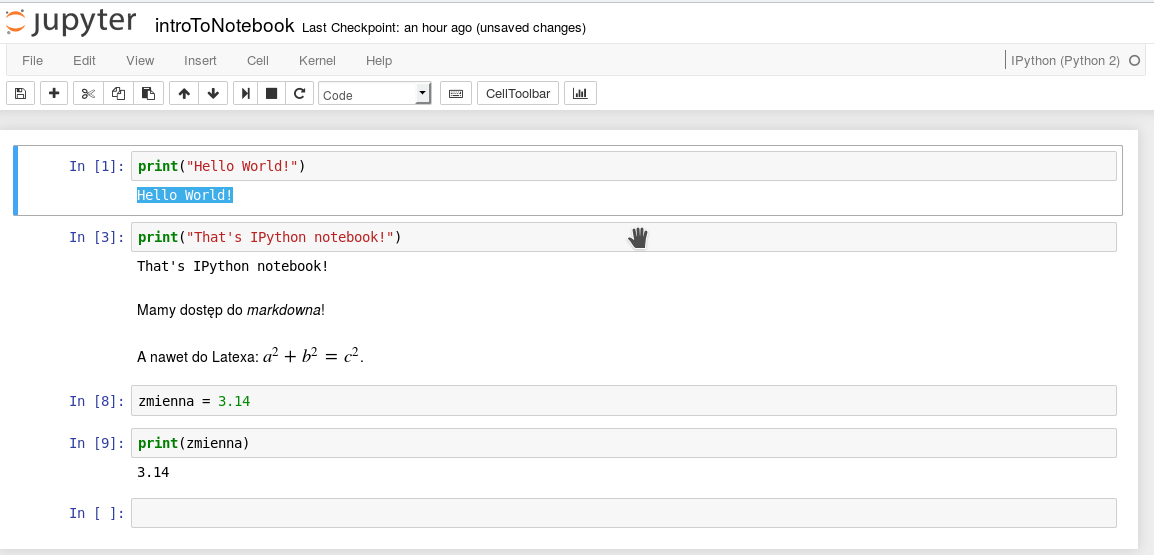
\includegraphics[width=10cm]{zad1}
    \caption{Wypełniony arkusz wprowadzający.}
  \end{figure}
\end{center}

\end{document}
